\chapter{Methods}

\section{The data}
PLease tell where is the data come from, a little brief of company can be put here.

\section {Mhd Zulfikar Akram Nasution / 1164081}
\subsection {Teori}
\begin{enumerate}
\item Random Forest
\par
Ramdom Forest adalah hutan yang acak, dimana maksudnya yaitu terdapat banyak pohon-pohon yang mana disetiap pohon tersebut memiliki atribut yang berbeda-beda, random forest disebut juga kumpulan pohon-pohon keputusan. contoh random forest seperti gambar 3.1
\begin{figure}[ht]
\centering
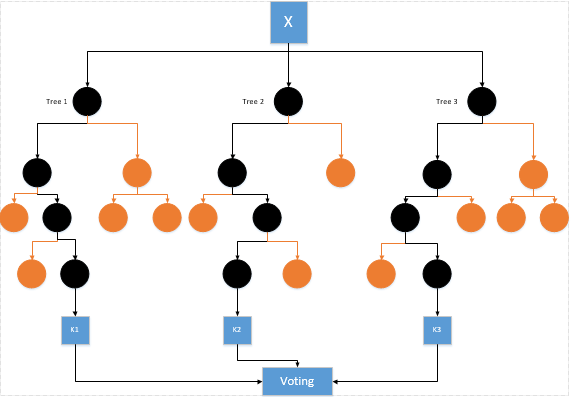
\includegraphics[scale=0.6]{figures/RF/1_1.png}
\caption{Random Forest}
\end{figure}
\item Cara membaca dataset kasus
\begin{itemize}
\item Buka aplikasi spyder untuk membuka dan membaca kodingan dataset
\item Kemudian buat  variable imgatt untuk memasukkan atribut label
\item Lalu uji coba kodingan untuk mengetahui apa hasil dari dataset tersebut
\item imgatt.head() untuk melihat sebagian data awal
\item .shape untuk melihat jumlah data
\item .pivot untuk merubah atribut menjadi kolom
\par
Dengan menguji coba kodingan yang ada pada spyder kita akan dapat membaca dataset yang ada.
\end{itemize}
\item Cross Validation
\par 
Cross Validation adalah sebuah metode statistik yang digunakan untuk mengevaluasi kinerja model, dimana data dipisah menjadi dua subset yaitu data proses pembelajan dan data evaluasi atau validasi.
\item Arti 44 persen pada RF, 27 persen pada Decission Tree, dan 29 persen pada SVM.
\begin{itemize}
\item 44 persen pada Random Forest adalah menjunjukkan hasil yang sempurna pada keputusan yang diambil, biasanya hasil keputusan yang dicapai sekitar 42-44 persen.
\item 27 persen pada Decission Tree adalah menunjukkan hasil keputusan pada tiap-tiap tree dari dataset yang ada.
\item 29 persen pada SVM menunjukkan hasil keputusan dengan klasifikasi dari dataset yang ada.
\end{itemize}
\item Confusion Matrix
\begin{itemize}
\item Pertama import confusion matrixnya
\item Kemudian Plot confusion matrix
\item Lalu sesuaikan plotnya dengan nama data yang ada
\item Setelah itu plot kembali
\end{itemize}
\par
Contoh hasil connfusion matrix pada gambar 3.2
\begin{figure}[ht]
\centering
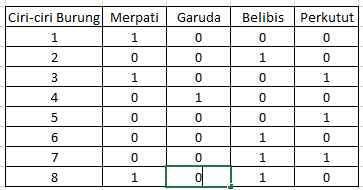
\includegraphics[scale=0.9]{figures/RF/1_2.png}
\caption{Confusion Matrix}
\end{figure}
\item Voting
\par
Voting adalah hasil akhir dari keputusan yang ada pasa setiap pohon di random forest, maksudnya ialah setiap keputusan yang telah dikumpulkan maka akan di voting bahwa hasil tersebut adalah hasil yang benar. Misalnya kita dapat lihat pada gambar 3.3 yaitu dari beberapa ciri-ciri yang ada dapat di voting atau disimpilkan hasil yang paling banyak dimiliki oleh burung belibis, sehingga dapat disimpulkan bahwa dari ciri- tersebut ialah merupakan ciri-ciri dari burung belibis. 
\begin{figure}[ht]
\centering
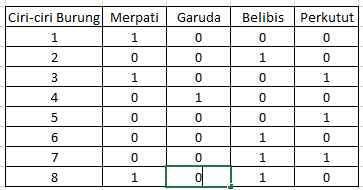
\includegraphics[scale=0.9]{figures/RF/1_2.png}
\caption{Voting}
\end{figure}

\end{enumerate}

\section{Method 1}
Definition, steps, algoritm or equation of method 1 and how to apply into your data
\section{Method 2}
Definition, steps, algoritm or equation of method 2 and how to apply into your data